\documentclass[12pt,a4paper,fleqn]{article}

\usepackage[utf8]{inputenc}
\usepackage[T1]{fontenc}
\usepackage{parskip}
\usepackage{amsmath, amssymb, graphicx, xcolor, array, multirow}
\usepackage{tcolorbox, nccmath}
\graphicspath{{/Users/econhead/NOTES/Microeconomics/MicroClassNotes/13_10_2024/Figures/}}
\setlength{\arrayrulewidth}{0.5mm} %table border thickness
\setlength{\tabcolsep}{18pt} %gap before text starts
\renewcommand{\arraystretch}{1.5} %cell height scaling
\usepackage{fancyhdr}
\setlength{\headheight}{15.6pt}
\pagestyle{fancyplain}
\fancyhead[L]{Laxman Singh}
\fancyhead[R]{\today}
\usepackage{float}
\floatstyle{boxed}
\restylefloat{figure}

\author{Laxman Singh}
\date{\today}
\title{Mixed Strategy Nash Equilibrium}     

\begin{document}
  \section{Mixed Strategy Nash equilibrium}
   \subsection{Battle of Sexes}
   \begin{tabular}{|c|c|c|c|b{3cm}|}
    \hline
       & M     & S     & \(\left( \frac{1}{2},\frac{1}{2} \right)\) & ($q,1-q$) \\ \hline
     M & (2,1) & (0,0)  & \(1,\frac{1}{2}\)  &  \(2q,q\)       \\ \hline
     S & (0,0) & (1,2) & \(\frac{1}{2},1\)   &  \((1-q),2(1-q)\) \\  \hline
    \(\left( \frac{1}{2},\frac{1}{2} \right)\)& \(1,\frac{1}{2}\)   &\(\frac{1}{2},1\) & \(\frac{3}{4},\frac{3}{4}\) & \\ \hline
     ($p,1-p$) & \(2p,p\)    & \((1-p),2(1-p)\) &   &\((2pq+(1-p)(1-q)),(pq+2(1-p)(1-q))\)  \\ \hline
    \end{tabular}
    
    Row player(Wife) plays the mixed strategy \((p,1-p) \ \text{s.t.} \quad p \in [0,1]\).
    
    Column player(Husband) plays the mixed strategy \((q,1-q) \ \text{s.t.} \quad q \in [0,1]\)  
   \begin{flalign*}
        A_{1}&=\left[ 0,1 \right] , A_{2}=\left[ 0,1 \right] \\
        U_{W}(p,q)&=pq+2(1-p)(1-q)=p(2q)+(1-p)(1-q)\\
        U_{H}(p,q)&=2pq+(1-p)(1-q)=q(p)+(1-q)(2(1-p))\\
        BR_{W}(q)&=\begin{cases}
            1 & \text{if} \quad 2q>1-q\leftrightarrow q>\frac{1}{3}\\
            0 & \text{ if} \quad 2q<1-q\leftrightarrow q<\frac{1}{3}\\
            \left[ 0,1 \right]   & \text{if} \quad 2q=1-q\leftrightarrow q=\frac{1}{3}
        \end{cases}\\
        BR_{H}(p)&=\begin{cases}
            1 & \text{if} \quad p>2(1-p)\leftrightarrow p>\frac{2}{3}\\
            0 & \text{ if} \quad p<2(1-p)\leftrightarrow p<\frac{2}{3}\\
            \left[ 0,1 \right] & \text{ if} \quad p=2(-p)\leftrightarrow p=\frac{2}{3}\\
        \end{cases}
   \end{flalign*}    
   So the mixed strategy nash equilibrium strategy in this game is \((p,q)=(\frac{2}{3},\frac{1}{3})\)  
      \begin{figure}[ht!]
       \centering
       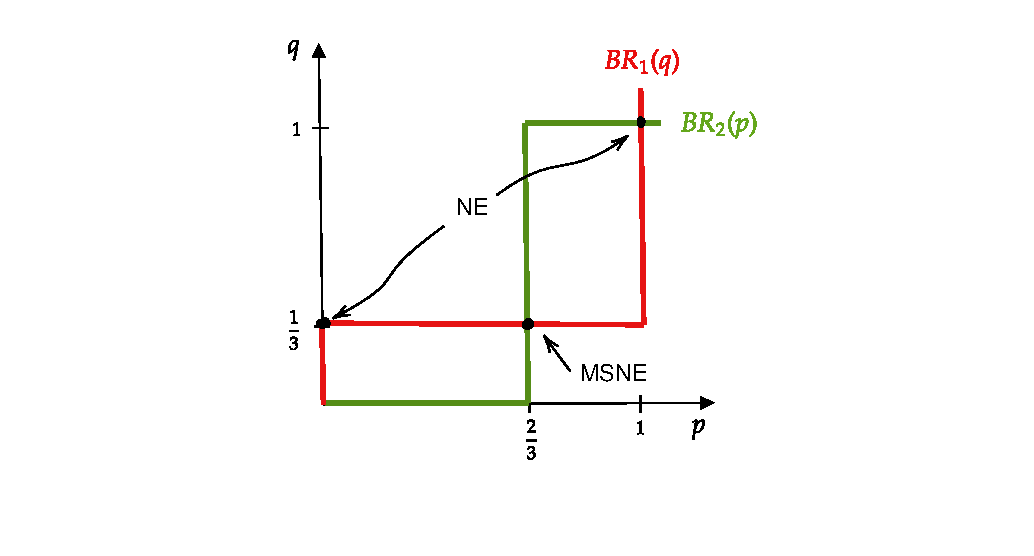
\includegraphics[scale=0.6]{MSNE.pdf}
       \caption{MSNE in Battle of Sexes}
       \label{Label}
    \end{figure}
   
    \subsection{Bargaining Game @3883}
    Two players negotiate over the price of a painting in which player \(1\) is the seller and quotes a price \(p \in \left[ 0,100 \right] \) and player 2 is the buyer with the following attributes;   
  
  \begin{fleqn}
   \begin{align*}
    N&=\{1,2\}\\
    T&=\{(p,D) \in \mathbb{R}_{+} \times \{A,R\}\}\\
    \mathcal{P}(\phi)&=1\\
    \mathcal{P}(p)&=2 \quad \forall p \in \mathbb{R}_{+}\\
    U_{1}(p,A)&=p , U_{2}(p,A)=100-p\\
    U_{1}(p,R)&=0 , U_{2}(p,R)=0\\
   \end{align*}
   Now player 2 will accept is \(100-p \geq 0\) that gives us the following best response function of player \(2\)   
   \begin{align*}
    BR_{2}(p)=\begin{cases}
        \mathrm{Accept} \quad \text{if } \quad p<100\\
        \mathrm{Reject}  \quad \text{if}   \quad p>100\\
        \mathrm{Accept}\quad  \text{if} \quad p=100\\
    \end{cases}
   \end{align*}
 \end{fleqn}
 and given this Best Response function of player \(2\), player \(1\) chooses \(p=100\) to maximize his payoff, which gives us our SPE. 

 Now,

 Strategy Set (or Choice Set) of Player 1 is \(S_1=\mathbb{R}+\) i.e. player 1 can offer any non-negative price \(s_1 \in S_1\).
    Strategy Set (or Choice Set) of Player 2 is \(S_2=\left\{s_2 \mid s_2: \mathbb{R}_{+} \rightarrow\{\right.\) Accept, Reject \(\left.\}\right\}\) i.e. player 2 chooses a function \(s_2 \in S_2\).
    Payoffs are represented by \(u_i: S_1 \times S_2 \rightarrow \mathbb{R}\) :
   \begin{align*}
    \begin{aligned}
     & u_1\left(s_1, s_2\right)= \begin{cases}s_1 & \text { if } s_2\left(s_1\right)=\text { Accept } \\
     0 & \text { otherwise }\end{cases} \\
     &  u_2\left(s_1, s_2\right)= \begin{cases}100-s_1 & \text { if } s_2\left(s_1\right)=\text { Accept } \\
     0 & \text { otherwise }\end{cases}
    \end{aligned}
   \end{align*}
   
   In the strategic form of this game and there are infite Nash equilibria in this game, two such NE strategy profiles are;
    \begin{itemize}
     \item \(s_{1}=100,s_{2}(s_{1})=\mathrm{Accept} \quad \text{if} \quad s_{1}\leq 100\)
     \item \(s_{1}=100,s_{2}(s_{1})=\mathrm{Accept} \quad \text{if} \quad s_{1}= 100\)
    \end{itemize}

 \subsection{More games}
 Suppose there are \(n\) people in a locality and a crime has been committed in this locality, every person has the same action set and the players are symmetric;

 \begin{fleqn} 
 \begin{equation*}
   \begin{split}
    A_{i}=\{\text{Report},\text{Don't Report}\} \\
   u_{i}(\mathrm{Report},a_{2},a_{3},\ldots,a_{n})=v-c \quad v>0, 0<c<v\\
   u_{i}(\mathrm{Don't \ Report,a_{2},a_{3}},\ldots,a_{n})= v \quad \text{if} \quad \exists \quad i \neq 1 \quad \text{s.t.} \ a_{i}=\text{Report}\\
    u_{i}(\mathrm{Don't \ Report},\ldots,\mathrm{Don't \ Report})=0\\
   \end{split}
 \end{equation*}
\end{fleqn} 
 Only one player reports and others do not report from the set of al players is a pure starategy Nash Equilibrium.
 
 Now, let us assume that players randomize their actions by the probability 
 \(\left( p,1-p \right) \) then, in order for any player to be indeifferent between randomizing and not randomizing between reporting and not reporting the crime, the following must hold;
 \begin{align*}
  v-c&=(1-p)^{n-1}(0)+(1-(1-p)^{n-1})(v)\\
  v-c&=v-v(1-p)^{n-1}\\
  (1-p)^{n-1}&=\frac{c}{v}\\
  1-p&=\left( \frac{c}{v} \right)^{\frac{1}{n-1}}\\
  p&= 1- \left( \frac{c}{v} \right)^{\frac{1}{n-1}}\\  
 \end{align*}  
\end{document}